%http://www.slideshare.net/boricles/linguistic-resources-enhanced-with-geospatial-information
In this section we present the specialisation of the Linked Data Life Cycle presented in \cite{Villazon_2011} applied to linguistics resources enhanced to geospatial information.

\subsection{Linguistics Resources}\label{sec:lr}

Our initial data source consisted of a spreadsheet containing GPS and lexical information for a variety of languages in the Dogon family, spoken in West Africa, and in particular in Mali. The information was gathered by linguists, and %is in publication elsewhere. 
In particular, these fields were gathered for each datapoint: language family, family code, language group, language group code, language autonym, dialect code, ISO 639-3 code, country code, village name, major cite, population, latitude, longitude, social information, images, image descriptions, video, video transcription, and a comment on the language. This means that each data point had a particular GPS mapping, which corresponded roughly to a local village or town. The initial goal of this dataset was to understand the spread, diversity, and phylogenetic origins of Dogon languages. The classification of Dogon is unclear, although there is substantial amounts of work in this area. 

%\cite{Bertho1953, Meillet_etal1952, Naden1989, Calame-Griaule1956, Calame-Griaule1978, Timbine1987, Bender-Samuel1971, Manessy1981, BendorHaretll1989, Galtier1993,Plungian1995, WilliamsonBlench2000, Lewis2009}

%Steve going to need your help here. 

\subsection{Specification}
In order to accurately model data according to the representations set forth by the communities involved in the Semantic Web, a specification must be laid out. A specification is a specific set of requirements that need to be satisfied by a resource. Here, we are concerned with converting plain text data from a spreadsheet into RDF. In order to be properly specified, we need to plan how the information will be represented. In order to fit the Linked Open Data paradigm described in \ref{sec:intro}, all referred entities must be designated using a Uniform Resource Identifier (URI). Each URI needs to be resolvable over HTTP; that is, they need to be able to be looked up and referred to by a web page. This is the base URI structure. Vocabulary elements - what constitutes the language used to refer to different objects from this base URI - must also be defined, just as instances - particular cases of an element - need to be. The finished specification for our data set - which, at heart, is little more than the links needed to refer to the data once it is loaded into an ontology online, is described below. 

%Boris, this doesn't seem to be accessible at the moment. Thoughts?

\subsubsection{URI design}
All the resources in our dataset are defined using a URI. URIs have been designed with simplicity, stability and manageability in mind, following common guidelines for their effective use\footnote{\url{http://www.w3.org/TR/cooluris/}},\footnote{\url{http://www.w3.org/Provider/Style/URI}}, \footnote{\url{http://www.w3.org/TR/chips/}}. 

\subsubsection{Base URI structure}

\noindent\surl{http://linguistic.linkeddata.es/}
%This is a just an index to the web page. Unless that's what you mean to show? 

\subsubsection{Vocabulary elements}

\noindent\surl{http://linguistic.linkeddata.es/ontology/{property|class}} \\

\noindent For example: \\
\surl{http://linguistic.linkeddata.es/ontology/officialName}
%This doesn't work. 

\subsubsection{Instances}

\noindent\surl{http://linguistic.linkeddata.es/dataset/resource/{r. type|r. name}}\\

\noindent For example: \\
\surl{http://linguistic.linkeddata.es/mlode/Village/Sokoura}
% This doesn't work. 

\subsection{Modelling}
The development of the linguistics vocabulary, which covers the linguistic information stored in the resources described in section \ref{sec:lr}, was performed following an iterative approach based on the reuse of existing knowledge management resources for linguistics. In a nutshell we have reused the following vocabularies: 
\begin{itemize}
	\item GOLD\footnote{\url{http://linguistic-ontology.org}}, an ontology for descriptive linguistics.
	\item WGS84 Geo Basic Vocabulary\footnote{\url{http://www.w3.org/2003/01/geo/}}, for representing the geospatial data.	 
\end{itemize} 

Nevertheless, it was necessary to create some of our own terms. However, this work was largely trivial. %Right? Otherwise, we need to describe this. I'm not sure what the development of vocabulary has to do with anything. What does this mean? This isn't geared towards new researchers. 

\subsection{Generation}
Next, the RDF was generated within three main phases. This is the process by which the spreadsheet turns into a useable resource. Here, we describe each one of these phases:

\begin{enumerate}
	\item Importing the spreadsheet into MySQL database by using the MySQL importing tool.
	\item Defining a set of R2RML\footnote{R2RML is a standard RDB2RDF mapping language \url{http://www.w3.org/TR/r2rml/}} mappings among the MySQL database and RDF vocabulary elements.
	\item Executing the R2RML engine, morph\footnote{\url{https://github.com/boricles/morph}}, for generating the RDF instances from the MySQL database data by using the defined R2RML mappings.  
\end{enumerate}

\begin{figure*}[htb!p]
\centering
%\includegraphics[scale=0.45]{IMGS/detalle_bn.png}
%\includegraphics[width=0.70\textwidth]{IMGS/detalle.pdf}
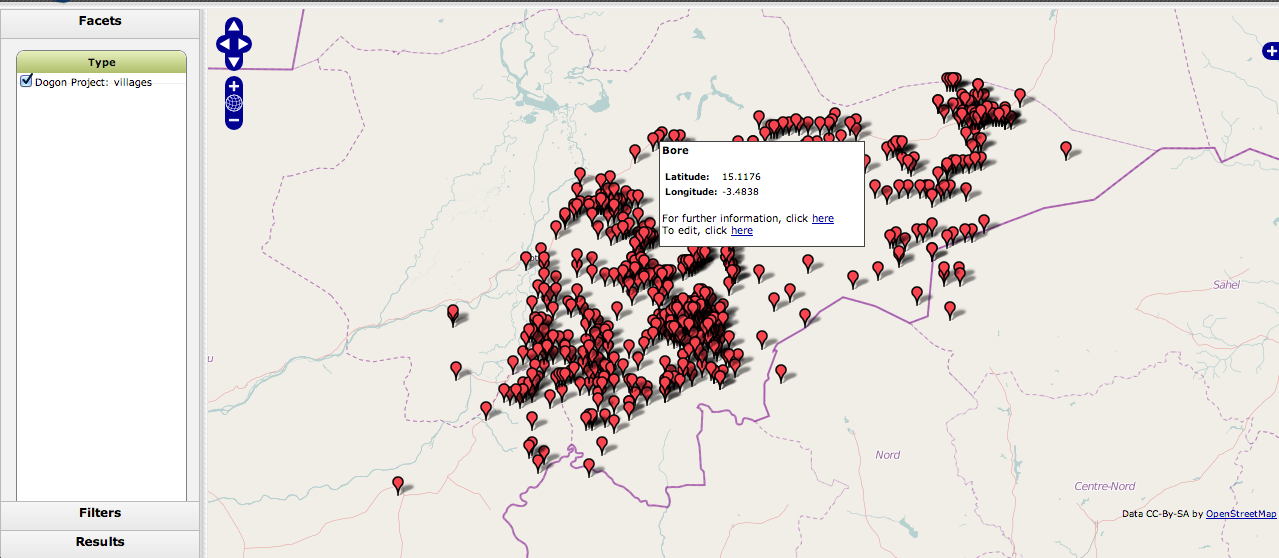
\includegraphics[width=0.99\textwidth]{img/map4rdf.png}
\caption{Visualization of the Dogon villages}
\label{fig:map4rdf}
\end{figure*}

\subsection{Publication}\label{sec:pub}
The generated RDF was then stored in Virtuoso\footnote{\url{http://virtuoso.openlinksw.com/}} open source version. Virtuoso is essentially the server, allowing the RDF data loaded in the Generation step above to be queried using an endpoint. Virtuoso integrates with Pubby\footnote{\url{http://www4.wiwiss.fu-berlin.de/pubby/}} to publish the results - Pubby is a fronted for endpoints, allowing users to query the data in the Virtuoso server using the SPARQL query language. Once Virtuoso and  Pubby are running on data that has been loaded in using the R2RML engine, all of the data is essentially available for humans and computers to read. At this point the data, if it has been specified correctly, if the URIs are HTTP resolvable and if the vocabulary followed set standards, the process of lifting data into the Semantic Web is practically done.  What's left is actually exploiting this data. 

\subsection{Exploitation}
The resultant dataset, following the previous steps, exposes the linguistics resources we first described enhanced with geospatial information, allowing for queries that otherwise require a lot of time by just looking at the original files. However, the data still hasn't been mapped - at best, SPARQL will return triples for any query. 

However, by extending the queries presented previously, we have built an application\footnote{\url{http://geo.linkeddata.es/map4rdf-dogon/}} for showing each of the Dogon villages on the map by using the tool map4rdf\footnote{\url{https://github.com/boricles/linked-data-visualization-tools}} \cite{deLeon_2012}. Figure \ref{fig:map4rdf} shows the application. At this point, each of the data points can be visualised. 


